Полный линейный коэффициент $\mu$ ослабления пучка $\gamma$-квантов при
прохождении через вещество равен сумме коэффициентов для всех трех рассмотренных
процессов. На рис. \ref{ris mu} изображены графики $\mu$ для различных
материалов.

\begin{figure}[h!]
  \centering
  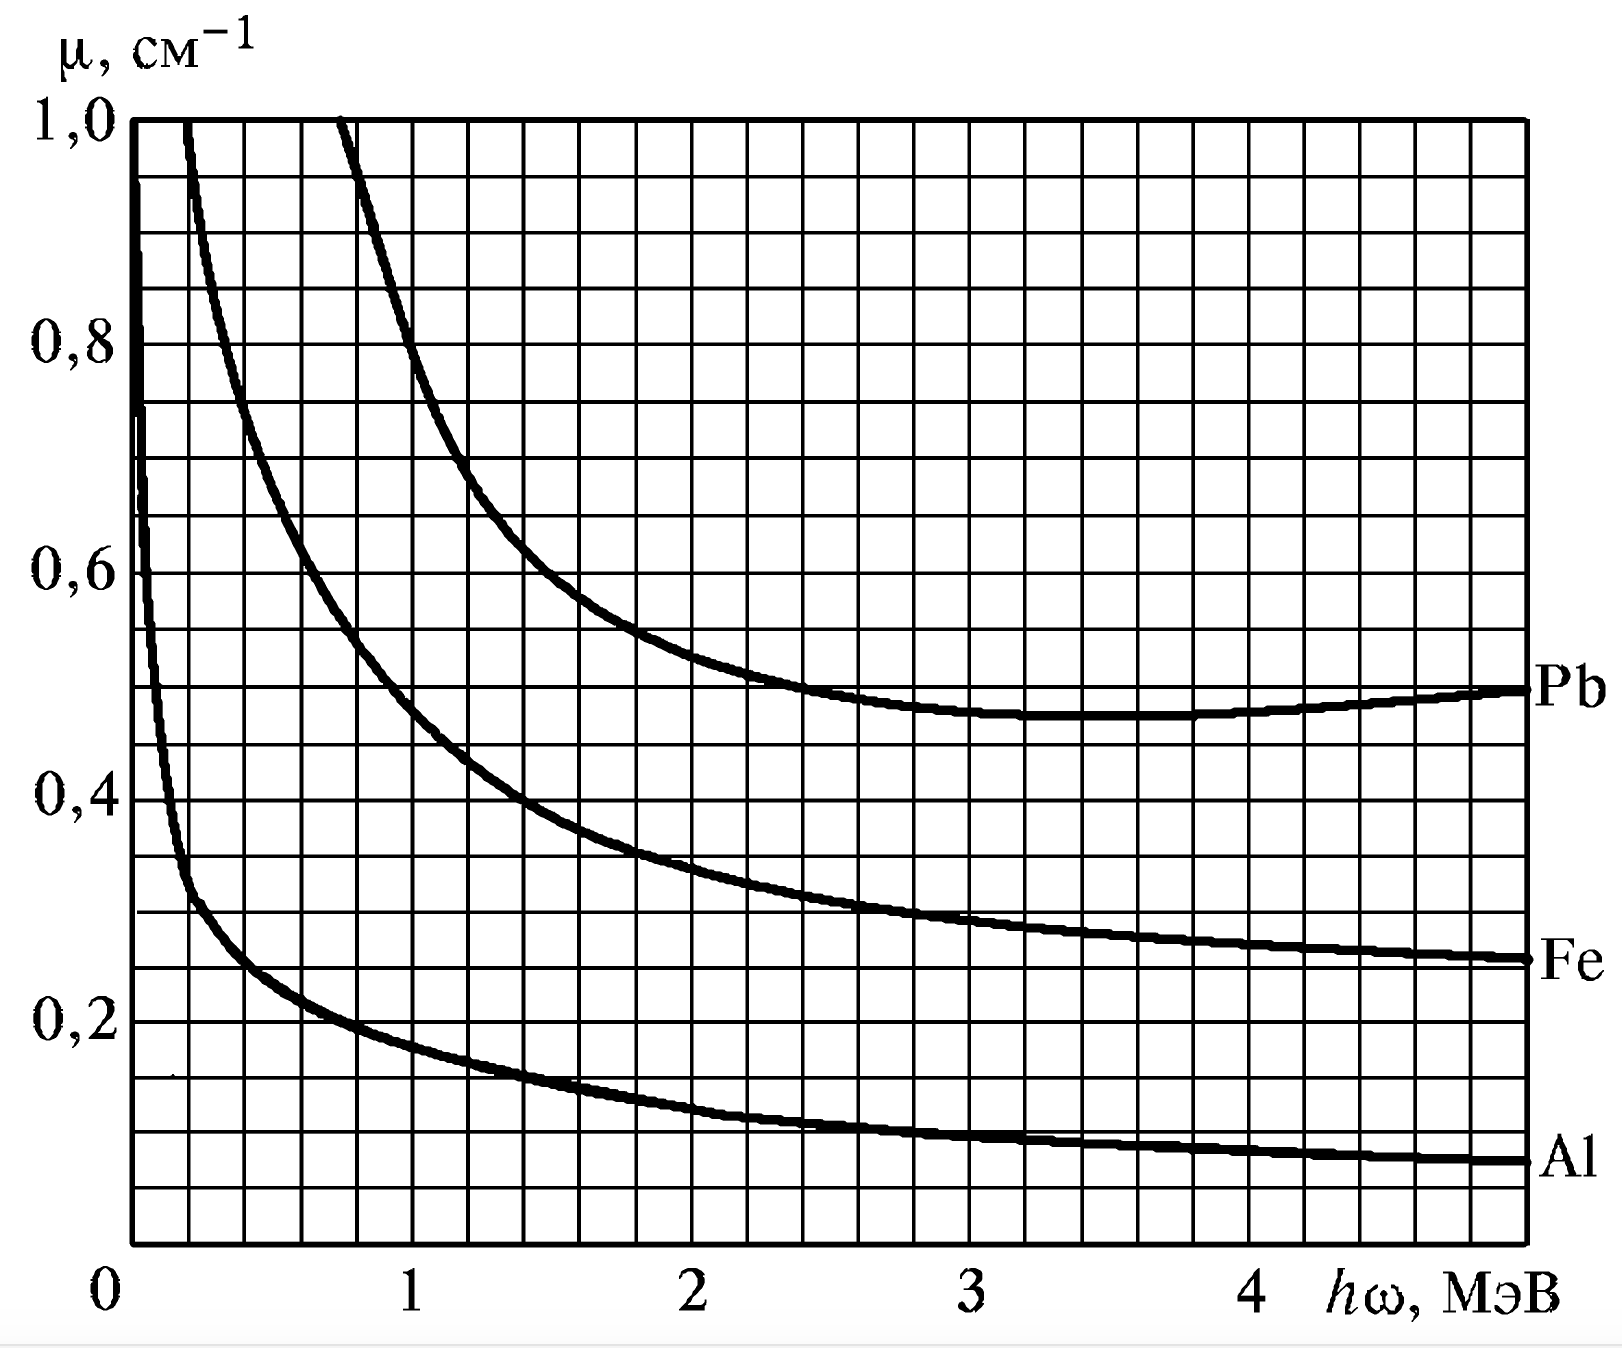
\includegraphics[width=0.6\linewidth]{mu}
  \caption{Полные коэффициенты ослабления потока $\gamma$-лучей в алюминии, железе и свинце}
  \label{ris mu}
\end{figure}

Обратимся вновь к формуле \eqref{I(mu)}. Ее нетрудно получить из теоретических
соображений. Рассмотрим опыты, поставленные в хорошей геометрии, т. е. в
условиях, когда исследуется прохождение сквозь вещество узкого параллельного
пучка $\gamma$-лучей. В этом случае не только фотоэлектрическое поглощение и
генерация пар, но и комптоновское рассеяние выводит $\gamma$-кванты из пучка.
Поэтому при прохождении через вещество меняется только количество, но не энергия
$\gamma$-квантов в пучке, так что коэффициент $\mu$, характеризующий поглощение
$\gamma$-квантов в веществе, не зависит от длины пути. Обозначим через $-dN$
число $\gamma$-квантов, выбывших из пучка на пути $dl$. Это число
пропорционально имеющемуся их числу $N$ и прой- денному пути $dl$. Имеем,
следовательно,

\begin{equation}\label{N}
-dN = \mu N dl \Rightarrow N = N_0 e^{-\mu l}
\end{equation}

т.е то же самое, что и формула \eqref{I(mu)}. В плохой геометрии, когда
рассеянные под небольшими углами $\gamma$-кванты остаются в пучке, их спектр с
прохождением вещества меняется, и формула \eqref{I(mu)}, вообще говоря,
неприменима. Эта формула, однако, работает и в этом случае лучше, чем можно было
бы ожидать. Причина хорошего согласия заключается в том, что $\gamma$-кванты с
энергией 1 -- 2 МэВ, потерявшие энергию из-за комптоновского рассеяния, быстро
выбывают из пучка из-за резкого увеличения сечений $\sigma_{\text{ф}}$ и
$\sigma_{\text{к}}$.

В данной работе коэффициент ослабления $ \mu $ измеряется в хорошей геометрии.
Из формулы \eqref{I(mu)} или \eqref{N} имеем

\begin{equation}\label{mu}
\mu = \dfrac{1}{l} \ln{\dfrac{N_0}{N}}
\end{equation}

Для определения коэффициента ослабления нужно, таким образом, измерить толщину
образца $l$, число падающих частиц $N_0$ и число частиц $N$, прошедших через
образец.